%%%%%%%%%%%%%%%%%%%%%%%%%%%%%%%%%%%%%%%%%%%%%%%%%%%%%%%%%%%%%%%%%%%%%%%%%%%%%%%%
%2345678901234567890123456789012345678901234567890123456789012345678901234567890
%        1         2         3         4         5         6         7         8

\documentclass[letterpaper, 10 pt, conference]{ieeeconf}  % Comment this line out if you need a4paper

%\documentclass[a4paper, 10pt, conference]{ieeeconf}      % Use this line for a4 paper

\IEEEoverridecommandlockouts                              % This command is only needed if 
                                                          % you want to use the \thanks command
\usepackage{subfigure}
\usepackage{cite}
\usepackage{amsmath,amssymb,amsfonts}
% \usepackage{algorithmic}
\usepackage{graphicx}
\usepackage{textcomp}
\usepackage{xcolor}
%\usepackage[numbers,sort&compress]{natbib}
\usepackage{algorithm} %format of the algorithm 
\usepackage{multirow} %multirow for format of table 
\usepackage{amsmath} 
\usepackage{gensymb}
\usepackage{mathtools}
\usepackage{forloop}
\usepackage{soul}

 
\usepackage{algorithmicx}  
\usepackage{algpseudocode}  

\usepackage{algorithm}  

\usepackage[UTF8]{ctex} 



\soulregister\cite7
\setlength{\textfloatsep}{5pt}

\overrideIEEEmargins                                      % Needed to meet printer requirements.

%In case you encounter the following error:
%Error 1010 The PDF file may be corrupt (unable to open PDF file) OR
%Error 1000 An error occurred while parsing a contents stream. Unable to analyze the PDF file.
%This is a known problem with pdfLaTeX conversion filter. The file cannot be opened with acrobat reader
%Please use one of the alternatives below to circumvent this error by uncommenting one or the other
%\pdfobjcompresslevel=0
%\pdfminorversion=4

% See the \addtolength command later in the file to balance the column lengths
% on the last page of the document

% The following packages can be found on http:\\www.ctan.org
%\usepackage{graphics} % for pdf, bitmapped graphics files
%\usepackage{epsfig} % for postscript graphics files
%\usepackage{mathptmx} % assumes new font selection scheme installed
%\usepackage{times} % assumes new font selection scheme installed
%\usepackage{amsmath} % assumes amsmath package installed
%\usepackage{amssymb}  % assumes amsmath package installed



\title{\LARGE \bf
基于强化学习和注意力机制的车辆换道研究
}


\author{沈炼成,林镇阳,韩立君 }% <-this % stops a space


\UseRawInputEncoding
\begin{document}



\maketitle
\thispagestyle{empty}
\pagestyle{empty}


%%%%%%%%%%%%%%%%%%%%%%%%%%%%%%%%%%%%%%%%%%%%%%%%%%%%%%%%%%%%%%%%%%%%%%%%%%%%%%%%
\begin{abstract}
这里是华丽丽的摘要


\end{abstract}


%%%%%%%%%%%%%%%%%%%%%%%%%%%%%%%%%%%%%%%%%%%%%%%%%%%%%%%%%%%%%%%%%%%%%%%%%%%%%%%%
\section{简介}

\section{任务描述与分析}

\subsection{任务描述}

整体任务为根据输入的车辆周围情况,借助深度强化学习算法得到高层的指令规划。再借助仿真器内部的运动规划器,将高层指令转化为具体的轨迹让底层控制器有效跟踪。最终实现汽车的超车换道。评价标准如下:
\begin{itemize}
    \item 尽可能少碰撞
    \item 尽量保持车道线内平稳行驶
    \item 速度越快越好
    \item 有前车阻挡能尝试安全换道
\end{itemize}

\subsection{仿真环境描述}
整体实验基于$highway\_env$开发,具有较强的灵活性。下面分别针对状态空间、动作空间等进行叙述。
\subsubsection{状态空间}
在环境中,状态空间可以选择底层的低维向量输入,也可以选择高维的图像输入和占用格作为输入。下面重点叙述使用低维向量输入和图片输入的基本情况。

当使用低维输入时,传入15辆车的坐标、速度、倾斜角度等信息表示出来,包括$x,y,vx,vy,cos_h,sin_h$。传入一个大小为$[15,7]$的数组。方便后面网络进行处理,其中第一行表示的是本车的的各种信息。

使用图片输入时,传入大小为$[600,150]$的图片,同时将图片转化为灰度图。由于一张图片难以获得车辆的完整信息(如速度、运动方向等难以推测),因此将过去4帧叠放在一起作为状态观测输入,便于从观测推出状态。

\begin{figure}[htb] %H为当前位置,!htb为忽略美学标准,htbp为浮动图形
    \centering %图片居中
    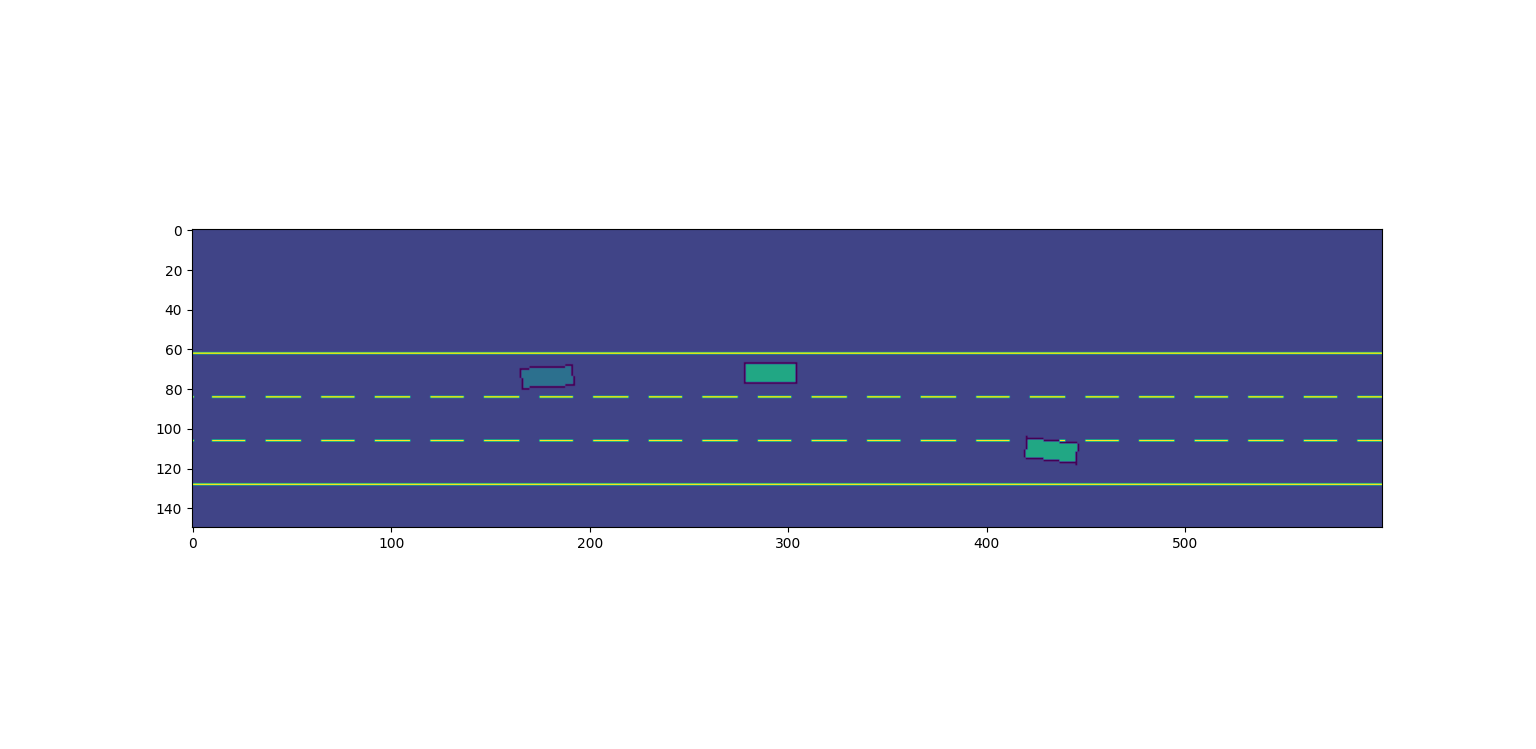
\includegraphics[width=0.5\textwidth]{fig/1.png} %插入图片,[]中设置图片大小,{}中是图片文件名
    \caption{图像输入} %最终文档中希望显示的图片标题
    \label{Fig.main1} %用于文内引用的标签
\end{figure}

后续实验证明,向量输入的归一化以及将两者信息整合同时输入可以显著提升换道效果。

\subsubsection{动作空间}
仿真环境可以将动作设置为连续的油门和方向盘角度,但连续空间训练收敛难度会增大。考虑到算力限制,因此使用离散动作进行控制,再将离散动作送入规划器中生成连续动作。在仿真器中,可以分为5个离散动作——左转、保持车道、右转、加速、减速。分别用动作$a_0$到$a_4$表征。这五个动作共同构成了仿真环境的动作空间,下层规划器根据决策指令对车辆动作进行规划控制。

\subsubsection{奖励设置}
环境中奖励设置较为灵活,主要分为三个部分,碰撞惩罚、车速奖励、靠右奖励。系统默认碰撞惩罚为-1,无碰撞为0。车速奖励为$r_v = 0.4\frac{(v_t-v_{min})}{(v_{max}-v_{min})}$其中,$v_{max} = 30m/s,v_{min}=20m/s$。此外还有靠右奖励,奖励系数为0.1。后面我们会讨论调整奖励系数对车辆的影响,实验发现,删除靠右奖励会导致车辆换道次数显著增加。

\subsection{任务分析}
根据任务需要我们设计强化学习算法,将低维或高维输入转化为离散的汽车换道决策指令。即首先需要对观测量进行提取推测,得到状态量。再将状态量作为输入得到动作。而近来深度强化学习的兴起让这两个环节可以直接联合训练,提升了学习效率。

在学习算法方面,我们采用了Dueling DDQN技术加入了一些训练技巧,能够有效提升收敛速度和训练稳定性。具体方法我们会在下节进行详细叙述,同时与之前的Dueling DQN,DQN进行比较,证明我们方法的有效性。同时针对输入,我们分别探讨了对于向量输入、图片输入和混合输入的效果。此外,针对不同奖励设置进行了消融实验。

\section{强化学习算法}
可以将超车换道问题转化为一个马尔可夫问题,由$<\mathcal{S},\mathcal{A},\mathcal{P},\mathcal{R},\gamma>$来表示,分别代表了状态空间、动作空间、转移概率、奖励函数、折扣因子。

根据前一节的分析,状态空间、动作空间、奖励函数均已得到。折扣因子$\gamma$设为0.99。不妨设$t$时刻的回报$G_t$为:
$$
G_t = \sum^{\infty}_{i=0}\gamma^ir_{t+i}
$$

$G_t$表示了从$t$时刻到结束的总的奖励,整个强化学习过程的目标即为最大化回报。但转移概率未知,因此采用无模型强化学习的方法,常用的无模型方法为Q学习算法。针对某个策略,定义$Q^\pi$为状态动作对好坏的评价标准,可以借助前面的回报定义为:

$$
Q^\pi = \mathbb{E}_\pi[G_t|s_t=s,a_t=a]
$$

同时使用经验回放池,使得训练数据满足独立同分布假设,以及充分利用过往探索经验,方便进行深度学习。使用目标网络,防止计算TD误差时目标变动导致更新困难。使用$\epsilon-greedy$算法,$\epsilon$值逐渐衰减,来平衡整个利用与探索的过程。整个DQN算法流程如下所示:

\begin{figure}[htbp] %H为当前位置,!htb为忽略美学标准,htbp为浮动图形
    \centering %图片居中
    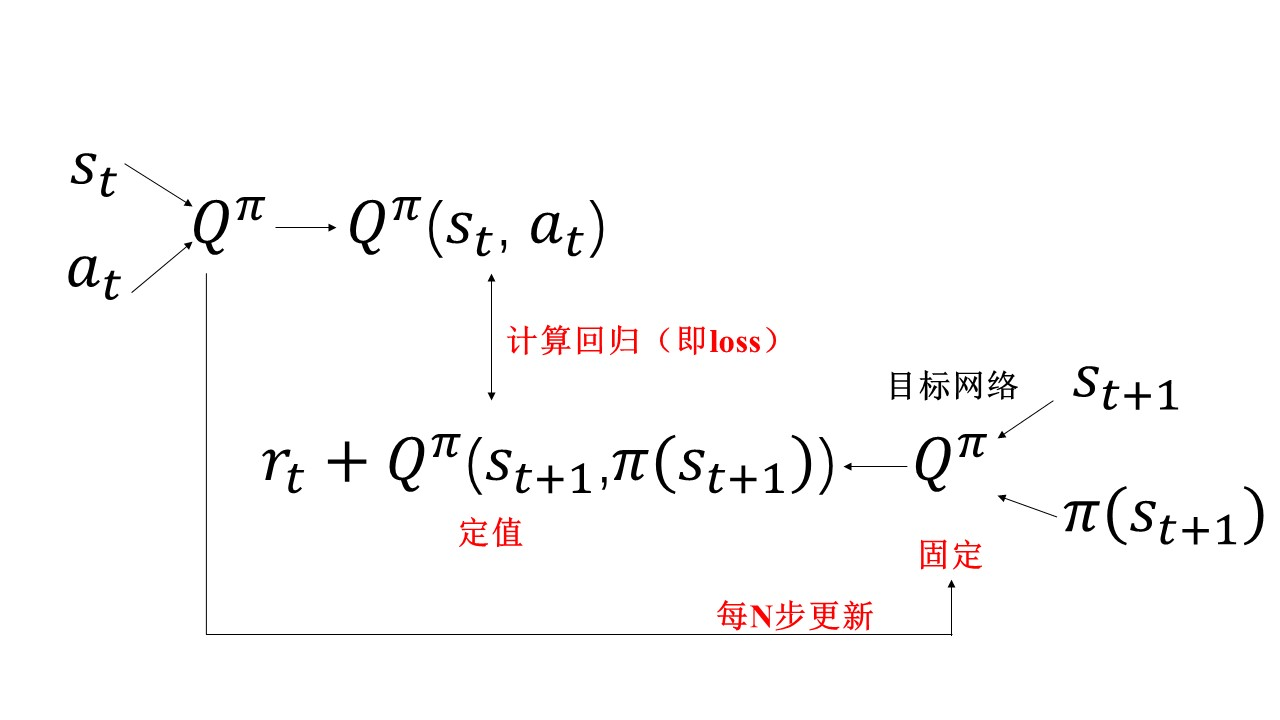
\includegraphics[width=0.5\textwidth]{fig/2.JPG} %插入图片,[]中设置图片大小,{}中是图片文件名
    \caption{DQN算法框架} %最终文档中希望显示的图片标题
    \label{Fig.main2} %用于文内引用的标签
\end{figure}


但是传统的DQN算法会存在Q值过高估计的问题,因此引入了Double DQN,将决策动作生成网络和状态动作对估值网络分开,可以一定程度缓解过估计问题。此外在训练数据中,很多状态并不需要估计每个动作的值,使用Q函数可能引入较多噪声。因此将Q函数分解为状态函数$V$和优势函数$A$最终$Q$值为两个函数的叠加。此外由于一个$Q$值可以有无数种分解方式,如果直接估计会导致难以收敛。因此对优势函数去均值保证分解的唯一性。最终$Q$值可以表示为:

$$
Q(s,a) = V(s)+(A(s,a)-\frac{1}{|\mathcal{A}|}\sum_{a'}A(s,a'))
$$

此外我们经过研究发现,获得终止信号有两种情况,撞车或达到仿真时间(50步)。但这两种情况实际上是不一样的。撞车后,我们不学习如何从撞车后恢复(相当于车辆已死亡),此时设为终止没有问题。但是只是到达了仿真步数,此时车辆其实是还可以正常行驶的,如果直接将该状态存为终止状态,会导致Q值的估计震荡不容易收敛。因此我们将原有算法进行了修改,加入了死亡判断。即每次动作得到终止信号时,会判断信号来源于撞车还是到达仿真步数,如果是来源于撞车,则存入经验池的$done=True$,否则仍设为$False$。具体算法如算法1所示。

\floatname{algorithm}{算法}

\begin{algorithm}[htbp]  
    \caption{加入死亡判断的Dueling DDQN算法}  
    \begin{algorithmic}[1] %每行显示行号  
            \State 初始化大小为$N$的经验回放池$D$,初始化随机选择概率$\epsilon$
            \State 使用随机参数$\theta$初始化动作价值函数$Q$
            \State 使用参数$\theta^-$初始化目标动作价值函数$\hat{Q}$,其中$\theta^- = \theta$
            \For{episode=1,episode<=M,episode++}
                \State 初始化状态序列$s_1={x_1}$
                \For{t=1,t<=T,t++}
                    \State 以$\epsilon$的概率进行随机动作选择$a_t$,否则选择$a_t = argmax_a \hat{Q}(s_t,a;\theta) $
                    \State 执行动作$a_t$得到奖励$r_t$和下一步的状态$s_{t+1}$,以及是否结束$d_t$
                    \If{$d_t==True$且发生了撞车}
                        \State $\hat{d_t}=True$
                    \Else
                        \State $\hat{d_t}=False$
                    \EndIf
                    \State 将数据$(s_t,a_t,r_t,s_{t+1},\hat{d_t})$存入经验回放池$D$中
                    \State 随机在经验回放池中选取一个$batch$的$(s_j,a_j,r_j,s_{j+1},,\hat{d_j})$
                    \State 令$y_j = 
                    \begin{cases}
                        r_j      &  \hat{d_j}=True \\
                        r_j+\gamma \max_{a'} \hat{Q}(s_{j+1},a';\theta^-)   & \mbox{其余情况}
                      \end{cases}
                    $
                    \State 设定损失函数为$(y_j-Q(s_j,a_j;\theta))^2$,采用随机梯度下降的方法更新参数$\theta$
                    \State 更新$\epsilon$,更新公式为$\epsilon_t =\epsilon_{max} - (\epsilon_{max}-\epsilon_{min})e^{-\frac{t_{sofar}}{n_{decay}}}$
                    \State 每$C$步令$\hat{Q} = Q$
                \EndFor
            \EndFor
    \end{algorithmic}  
\end{algorithm} 


\section{注意力机制}

\section{实验分析}



\addtolength{\textheight}{-1cm}   % This command serves to balance the column lengths
                                  % on the last page of the document manually. It shortens
                                  % the textheight of the last page by a suitable amount.
                                  % This command does not take effect until the next page
                                  % so it should come on the page before the last. Make
                                  % sure that you do not shorten the textheight too much.

%%%%%%%%%%%%%%%%%%%%%%%%%%%%%%%%%%%%%%%%%%%%%%%%%%%%%%%%%%%%%%%%%%%%%%%%%%%%%%%%



%%%%%%%%%%%%%%%%%%%%%%%%%%%%%%%%%%%%%%%%%%%%%%%%%%%%%%%%%%%%%%%%%%%%%%%%%%%%%%%%



%%%%%%%%%%%%%%%%%%%%%%%%%%%%%%%%%%%%%%%%%%%%%%%%%%%%%%%%%%%%%%%%%%%%%%%%%%%%%%%%
%\section*{APPENDIX}

%Appendixes should appear before the acknowledgment.

\section*{致谢}




%%%%%%%%%%%%%%%%%%%%%%%%%%%%%%%%%%%%%%%%%%%%%%%%%%%%%%%%%%%%%%%%%%%%%%%%%%%%%%%%

%References are important to the reader; therefore, each citation must be complete and correct. If at all possible, references should be commonly available publications.

\bibliographystyle{unsrt}
\bibliography{ref}%%我们的例子应该是\bibliography{cited}




\end{document}
